\documentclass[10pt,aspectratio=169]{beamer}

\useinnertheme[shadow=true]{rounded}
\useoutertheme{infolines}
\usecolortheme{whale}
\usecolortheme[RGB={245,128,37}]{structure}

\definecolor{bold}{RGB}{245,128,37}

\newcommand{\drawdownarrow}{\centering \vspace{0.05in}  {\LARGE $\downarrow$}  \vspace{0.05in}}
\DeclareMathOperator*{\argmin}{arg\,min}

\makeatletter
\setbeamertemplate{footline}
{
  \leavevmode%
  \hbox{%
  \begin{beamercolorbox}[wd=.333333\paperwidth,ht=2.25ex,dp=1ex,center]{author in head/foot}%
    \usebeamerfont{author in head/foot}\insertshortauthor~~\beamer@ifempty{\insertshortinstitute}{}{(\insertshortinstitute)}
  \end{beamercolorbox}%
  \begin{beamercolorbox}[wd=.333333\paperwidth,ht=2.25ex,dp=1ex,center]{title in head/foot}%
    \usebeamerfont{title in head/foot}\insertshorttitle
  \end{beamercolorbox}%
  \begin{beamercolorbox}[wd=.333333\paperwidth,ht=2.25ex,dp=1ex,right]{date in head/foot}%
    \usebeamerfont{date in head/foot}\insertshortdate{}\hspace*{8em}
    \insertframenumber\hspace*{2ex} 
  \end{beamercolorbox}}%
  \vskip0pt%
}
\makeatother
  
\usepackage{ragged2e}
%\usepackage{setspace}

\usepackage{forloop}
\usepackage[percent]{overpic}

\usepackage{extarrows}
\usepackage{tikz}
\usetikzlibrary{calc}
\usetikzlibrary{arrows}
\usetikzlibrary{decorations.markings}
\usetikzlibrary{positioning}

\usepackage{movie15}

\usepackage{animate}
\usepackage{amssymb}
\usepackage{color}
\beamertemplatenavigationsymbolsempty

\hyphenpenalty 10000
\exhyphenpenalty 10000
\widowpenalty 10000
\clubpenalty 10000

\usepackage[firstinits=true,style=verbose,maxnames=6,backend=bibtex]{biblatex}
\renewbibmacro{in:}{}
\bibliography{../../references/references}
\setbeamercolor{bibliography item}{use=normal text,fg=black}
\setbeamercolor*{bibliography entry title}{use=normal text,fg=black}
\setbeamercolor*{bibliography entry author}{use=normal text,fg=black}
\setbeamercolor*{bibliography entry journal}{use=normal text,fg=black}
\setbeamercolor*{bibliography entry note}{use=normal text,fg=black}

\DeclareCiteCommand{\footcite}{}{%
    \footnote{\printnames[author]{author}, \printfield{journaltitle}, \printfield{year}}} {\textsuperscript{,}}{}%

\DeclareCiteCommand{\footcitetext}{}{%
    \footnotetext{\printnames[author]{author}, \printfield{journaltitle}, \printfield{year}}} {\textsuperscript{,}}{}%    
    

\DeclareCiteCommand{\cite}{}{%
    \printnames[author]{author}, \printfield{journaltitle}, \printfield{year}} {;}{}%

\let\oldfootnotesize\footnotesize
\renewcommand*{\footnotesize}{\oldfootnotesize\tiny}


	

\graphicspath{ {images/} }

\title[Registration and Temporal Ordering of Images]{Registration and Temporal Ordering of Images \\ in Studies of Biological Development}

\author[C. Dsilva]{{\bf Carmeline~Dsilva}\inst{1},  Bomyi~Lim\inst{1}, Stanislav~Shvartsman\inst{1,2}, and Ioannis~Kevrekidis\inst{1,3}}
\institute[Princeton]{
  \inst{1}Department of Chemical and Biological Engineering\\
  \inst{2}Lewis-Sigler Institute for Integrative Genomics \\
  \inst{3}Program in Applied and Computational Mathematics \\
  Princeton University, Princeton, NJ 
  \\[1ex]
  \texttt{cdsilva@princeton.edu}
}
\date[July 2014]{15 July 2014}

\begin{document}

\begin{frame}[plain]
  \titlepage
  
\includegraphics[width=1in]{CSGF_horiz_1200x360}
  \hfill  
  
\includegraphics[width=1in]{PUsig2}
\end{frame}

\begin{frame}{Reconstructing Dynamics from Snapshots}

There are two types of data collection schemes% \\ when studying developmental dynamics

\begin{description}
\item[Longitudinal] The developmental trajectory of {\em a single organism} \\is monitored over time
\item[Cross-sectional] Samples from {\em many organisms} are collected; each organism contributes only a single snapshot from the developmental process
\end{description}

\vspace{0.1in}
\begin{center}
We will look at cross-sectional imaging data. %The tasks are
%then to \textcolor{bold}{register} and \textcolor{bold}{temporally order} the snapshots to obtain a representative developmental trajectory.

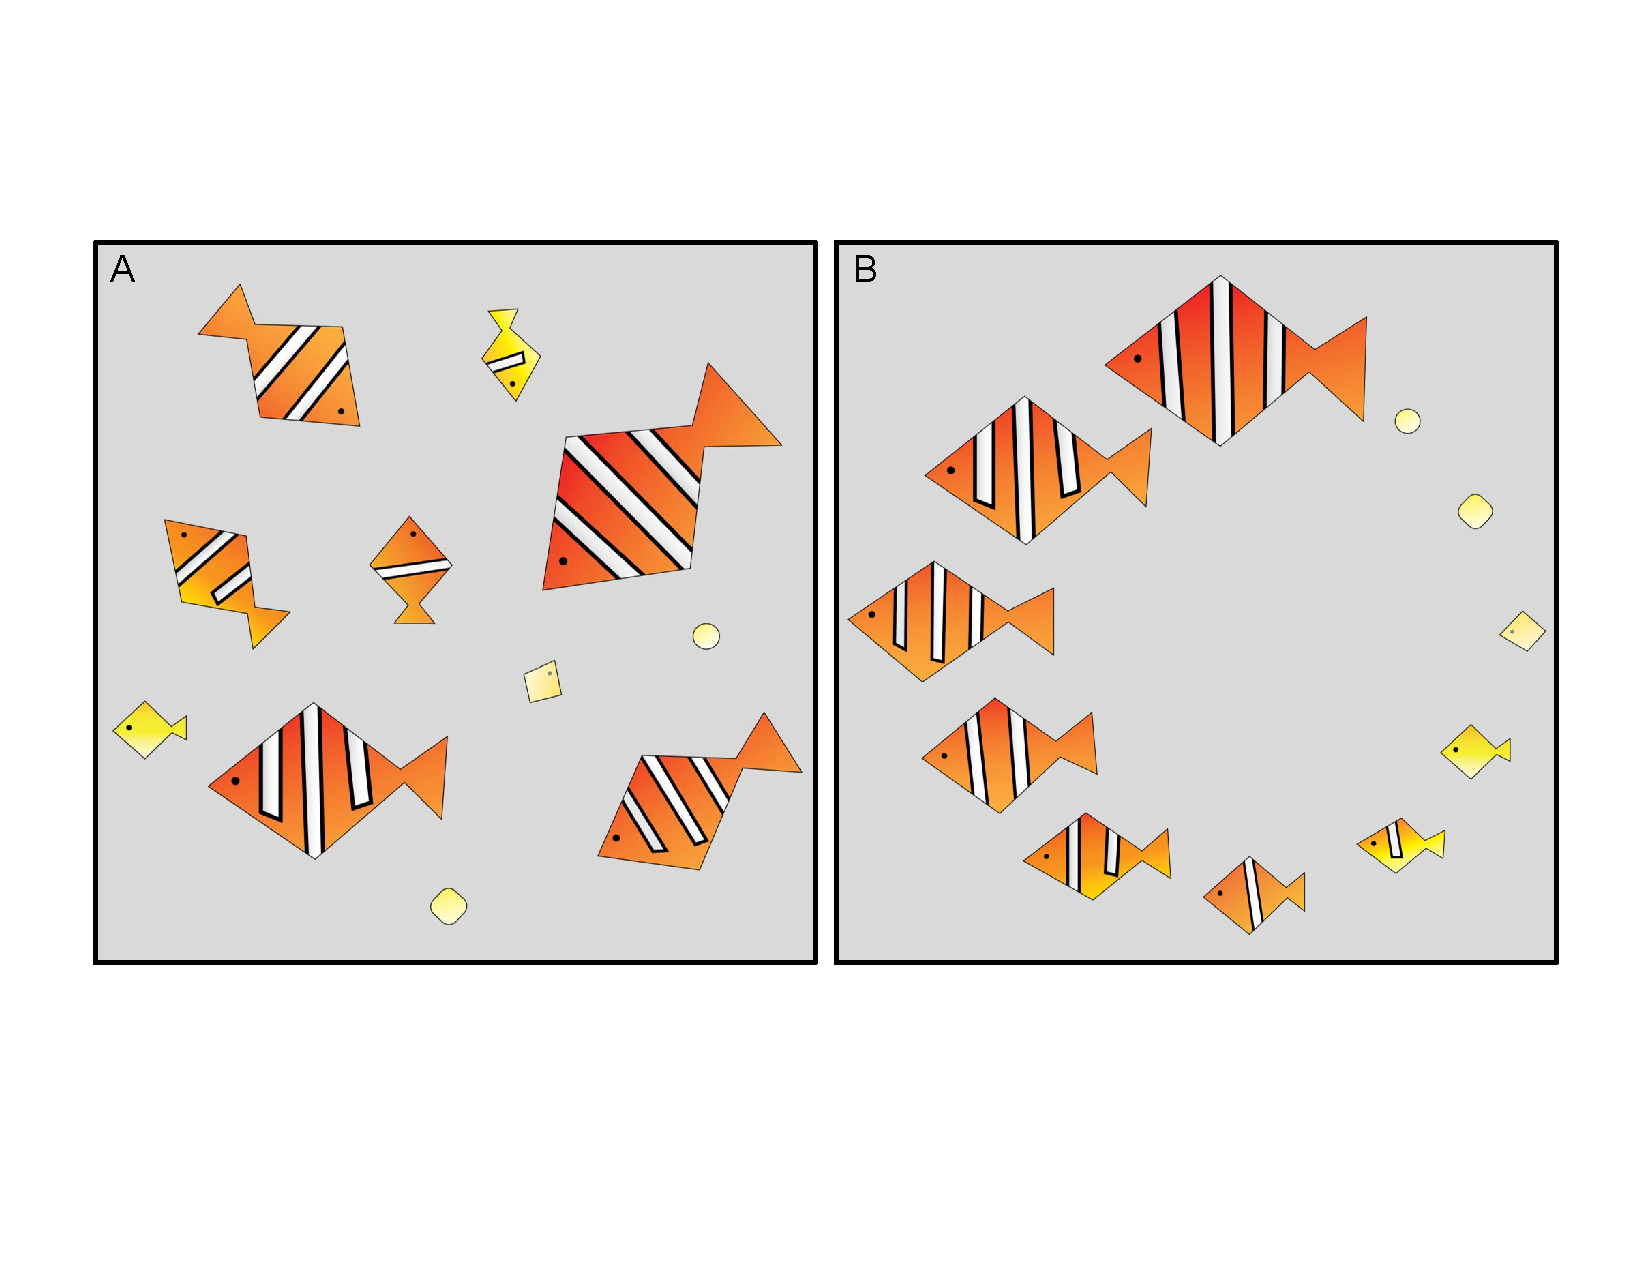
\includegraphics[width=2in]{fig1}

{\scriptsize A caricature of ordering cross-sectional data. \\
(Left) Fish, each in a different stage of development.  (Right) Fish, now registered and temporally ordered. \\ 
In this example, it is easy to order the data by hand. \par}
\end{center}

\end{frame}

\section{Experimental Setup and Data Collection}

\begin{frame}{Developmental Dynamics of {\em Drosophila} Embryogenesis}

\begin{minipage}[b]{0.7\textwidth}
\vspace{0.2in}
\begin{itemize}
%\item {\em Drosophila melanogaster} (common fruit fly) is one of the leading systems for studies in developmental biology (easy to grow, short generation time)
\item {\em Drosophila melanogaster} (common fruit fly) is a common model organism in developmental biology
\item We will look at {\em Drosophila} embryogenesis during the third hour of development
\end{itemize}
\end{minipage}
%
\hspace{0.2in}
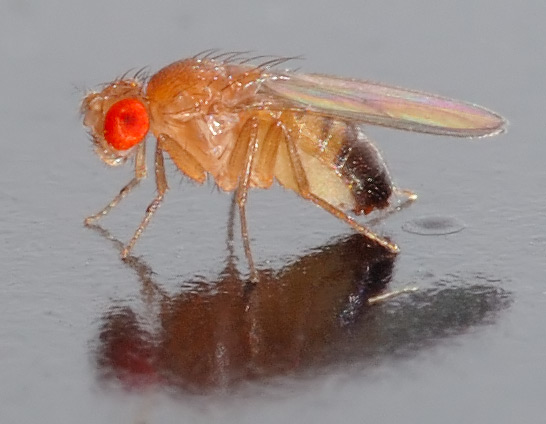
\includegraphics[width=0.7in]{drosophila_picture}

\vspace{0.3in}

\begin{center}
Images of {\em Drosophila} in the third hour of development


\begin{minipage}{0.3\textwidth}
\centering
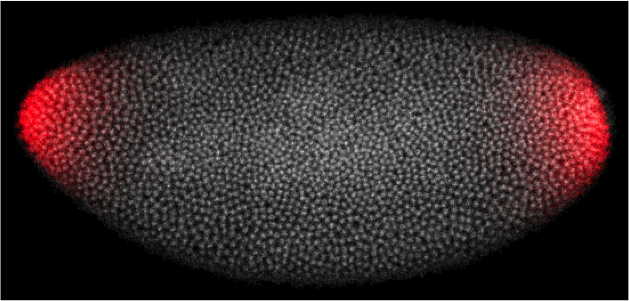
\includegraphics[width=1in]{longitudinal_5min}\\
{\em \scriptsize 5~min}
\end{minipage}
%
\begin{minipage}{0.3\textwidth}
\centering
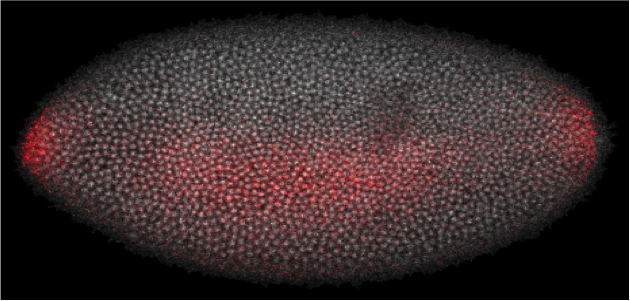
\includegraphics[width=1in]{longitudinal_25min}\\
{\em \scriptsize 25~min}
\end{minipage}
%
\begin{minipage}{0.3\textwidth}
\centering
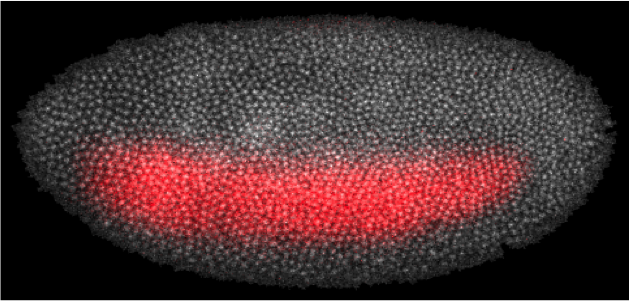
\includegraphics[width=1in]{longitudinal_45min}\\
{\em \scriptsize 45~min}
\end{minipage}

\end{center}

\begin{itemize}
\item Embryos are stained for important regulatory proteins (dpERK, shown in red) 

\item This staining cannot be done without first fixing the embryos
%\item It is impossible to obtain live images of the protein concentration profiles evolving in a single embryo.
\end{itemize}

\end{frame}

\begin{frame}{{\em Drosophila} Images}

\begin{center}
We will look at optical sections perpendicular to the long axis of the embryo

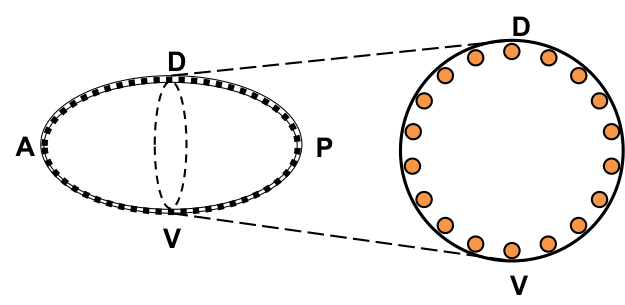
\includegraphics[width=2.5in]{drosophila_schematic}

\begin{tikzpicture}
\node[] (a) {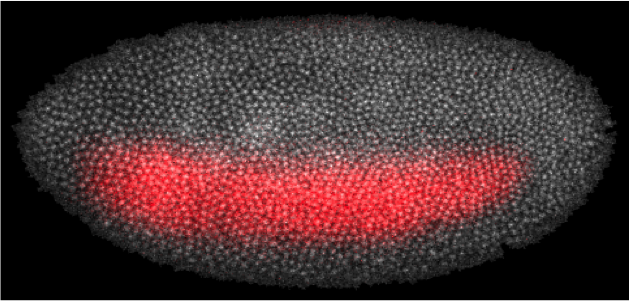
\includegraphics[width=1.3in]{longitudinal_45min}};
\node[right=0.4in of a] (b) {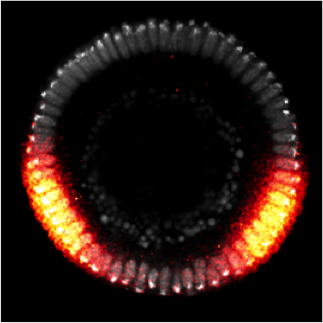
\includegraphics[width=0.7in]{DV_45min}};
\draw[->] (a.east) -- (b.west);
\end{tikzpicture}

The stripes now appear as peaks around the circumference of the embryo

\end{center}

\end{frame}

\begin{frame}{Data Collection}

\begin{center}
We use a microfluidic device \footcite{chung2010microfluidic} to easily obtain images of many embryos

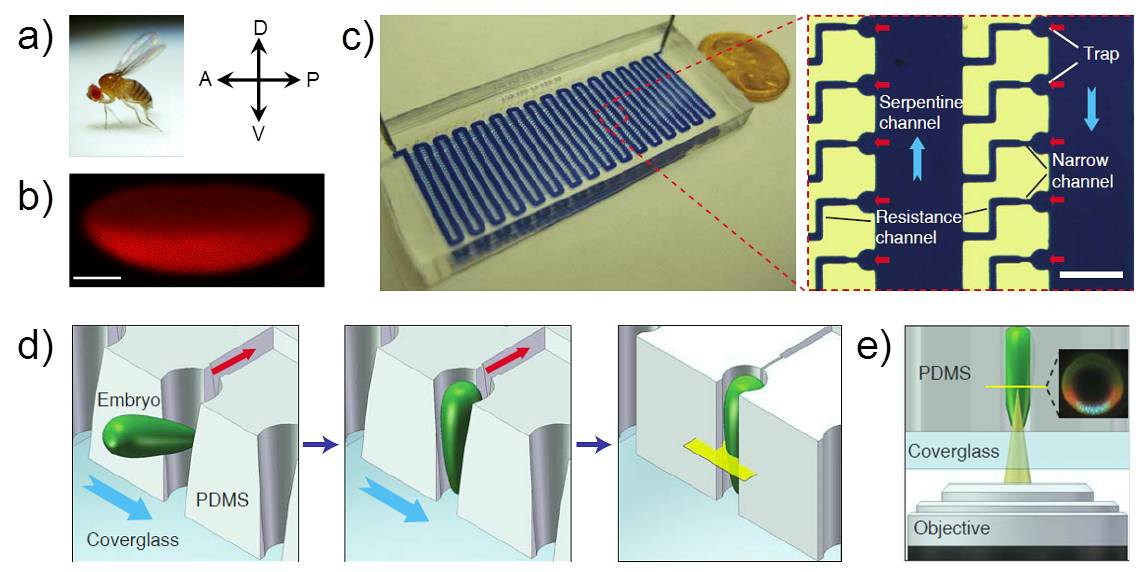
\includegraphics[width=3.5in]{drosophila_imaging_setup}

\vspace{0.15in}

\begin{minipage}[b]{1.1in}
\hfill
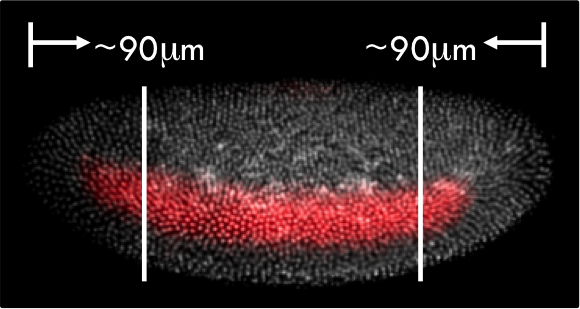
\includegraphics[width=0.9in]{imaging_depth}
\end{minipage}
%
\begin{minipage}[b]{0.65\textwidth}
We obtain images at a fixed depth (90~$\mu m$) \\from the tip of the embryo.

Each embryo is in a different rotational orientation.
\end{minipage}

\end{center}

\end{frame}

\begin{frame}{A Typical Data Set}
\begin{center}
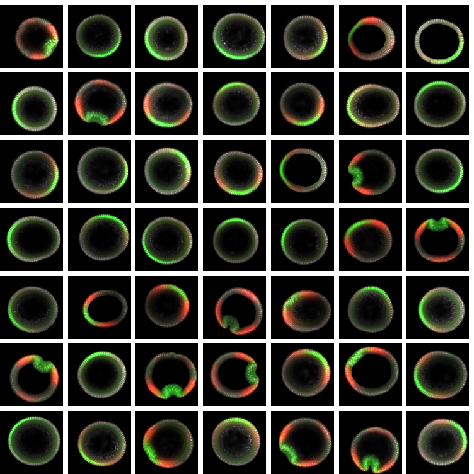
\includegraphics[width=2in]{fig2a}
\end{center}

\begin{itemize}
\item Each image is from a different embryo
\item Each embryo is stained for two different proteins\\ (Dorsal, in green, and dpERK, in red)
\item Each embryo is at a different (and unknown) developmental time
\item Each embryo is also at a different (and unknown) orientation
\end{itemize}
\end{frame}

\section{Mathematical Methods}

\begin{frame}{Mathematical Methods for Registration and Ordering}

\vspace{-0.1in}
\begin{center}
We will show how we can {\em automatically} register and order the images
\vspace{-0.05in}
\begin{tikzpicture}
\node(a) {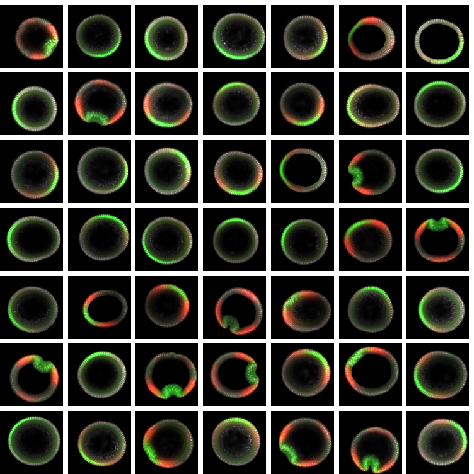
\includegraphics[width=1.5in]{fig2a}};
\node[right=0.2in of a] (b) {\includegraphics[width=1.5in]{VDM_data1_ordered}};
\draw[->] (a.east) -- (b.west);
\end{tikzpicture}
\end{center}

\vspace{-0.1in}
{\small 
\begin{description}
\item[Image registration] Angular synchronization \footcite{ singer2011angular}
{\scriptsize \em (other methods: templates \footcite{ahuja2007template}, feature extraction \footcite{zhao2003face, schindler2007inferring}) \par}

\item[Temporal ordering] Diffusion maps \footcite{coifman2005geometric} 
{\scriptsize \em (other methods: TSP \footcite{anavy2014blind}, MST \footcite{trapnell2014dynamics}) \par}

\item[Simultaneous registration and ordering] Vector diffusion maps \footcite{singer2012vector} 

\end{description}
 \par}
 
\end{frame}

\begin{frame}{Image Registration: Angular Synchronization}

\begin{itemize}
\item We want to align or {\em register} the images, \\since each image is taken in a different rotation
\item We do not know {\em a priori} what good image features are
\item We also do not know what a good template function is
\end{itemize}

\vspace{0.1in}
\begin{center}
\textcolor{bold}{What we can do:} compute pairwise alignments

\vspace{0.1in}
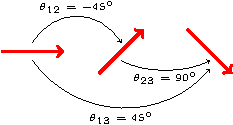
\includegraphics[width=2in]{synchronization1}
\end{center}

\end{frame}

\begin{frame}{Angular Synchronization: The Assumptions}

\begin{itemize}
\item Given data points $x_1, \dots, x_m$, we can compute $\theta_{ij}$, \\the angle needed to align $x_i$ to $x_j$.
\item We assume that each point $x_i$ is some rotated copy \\of an underlying signal $x_{true}$ (which we do not know).
\item Let $\theta_i$ denote the angle to rotate $x_{true}$ to $x_i$.
\item Therefore, $\theta_{ij} \approx \theta_i - \theta_j$, i.e., rotating $x_i$ to $x_j$ is like rotating $x_i$ to $x_{true}$, \\and then rotating $x_{true}$ to $x_j$

\end{itemize}

\begin{center}
\begin{tikzpicture}
\node[] (a) {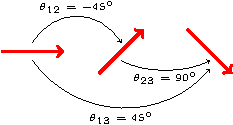
\includegraphics[width=2in]{synchronization1}};

\node[below=0in of a, text width=2in, align=center] (text) {Pairwise alignments $\theta_{ij}$ between set of vectors};

\node[right=0.5in of a] (b) {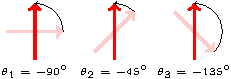
\includegraphics[width=2in]{synchronization2}};

\node[below=0in of b, text width=2in, align=center] (text) {Individual rotations $\theta_i$ for each vector};

\end{tikzpicture}

\end{center}

\end{frame}


\begin{frame}{Angular Synchronization: The Algorithm}

\begin{itemize}
\item We look at the matrix $H$ which contains information \\about all pairwise alignments
$$H = \begin{bmatrix}
e^{\theta_{11}} & e^{\theta_{12}} & \cdots & e^{\theta_{1m}} \\
e^{\theta_{21}} & e^{\theta_{22}} & \cdots & e^{\theta_{2m}} \\
\vdots & \vdots & \ddots & \vdots \\
e^{\theta_{m1}} & e^{\theta_{m2}} & \cdots & e^{\theta_{mm}} 
\end{bmatrix} $$
\item If our assumption holds ($\theta_{ij} \approx \theta_i - \theta_j$), then 
$$ H \approx \begin{bmatrix}
e^{\theta_1-\theta_1} & e^{\theta_1-\theta_2} & \cdots & e^{\theta_1-\theta_m} \\
e^{\theta_2-\theta_1} & e^{\theta_2-\theta_2} & \cdots & e^{\theta_2-\theta_m} \\
\vdots & \vdots & \ddots & \vdots \\
e^{\theta_m-\theta_1} & e^{\theta_m-\theta_2} & \cdots & e^{\theta_m-\theta_m} 
\end{bmatrix} =
\begin{bmatrix}
e^{\theta_1} \\
e^{\theta_2} \\
\vdots \\
e^{\theta_m}
\end{bmatrix}
\begin{bmatrix}
e^{-\theta_1} & e^{-\theta_2} & \cdots & e^{-\theta_m}
\end{bmatrix} $$
and the top eigenvector of $H$ gives us estimates of the optimal rotations
\end{itemize}

\end{frame}
%\begin{frame}{Angular Synchronization of {\em Drosophila} Images}
%
%\begin{center}
%\begin{tikzpicture}
%\node(a) {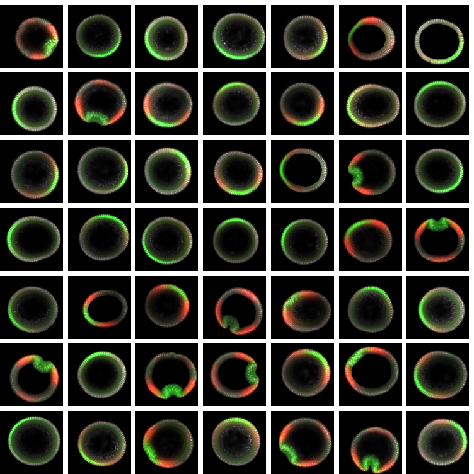
\includegraphics[width=2in]{fig2a}};
%\node[below=0in of a, align=center, text width=2in](text) {Images, unregistered and unordered};
%\node[right=0.5in of a] (b) {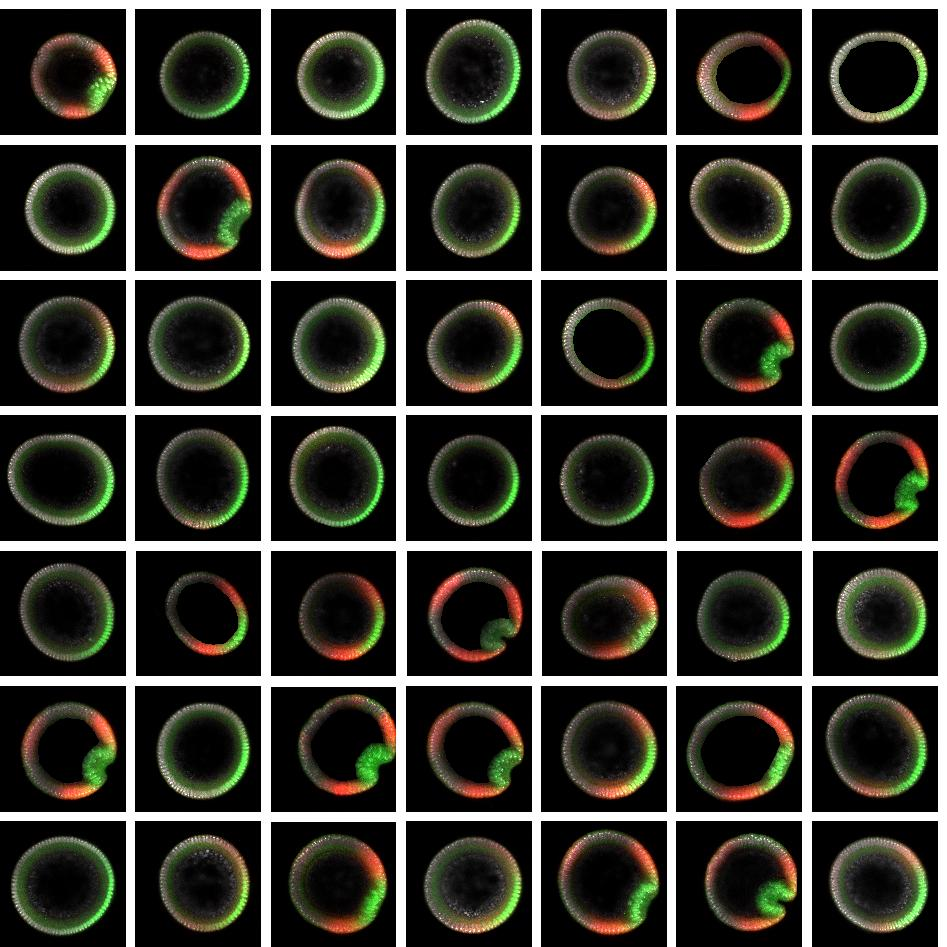
\includegraphics[width=2in]{images_angsynch}};
%\node[below=0in of b, align=center, text width=2in](text) {Images, registered using angular synchronization};
%\draw[->] (a.east) -- (b.west);
%\end{tikzpicture}
%\end{center}
%
%\end{frame}


\begin{frame}{Temporal Ordering: Diffusion Maps}

\begin{itemize}
\item We want to temporally order the (registered) images in time

\item Our images are high-dimensional vectors

\item We assume that our images lie on a one-dimensional (perhaps nonlinear) curve

\item We also assume that this curve is parameterized by time

\end{itemize}

\begin{center}
\begin{tikzpicture}

\node[] (a) {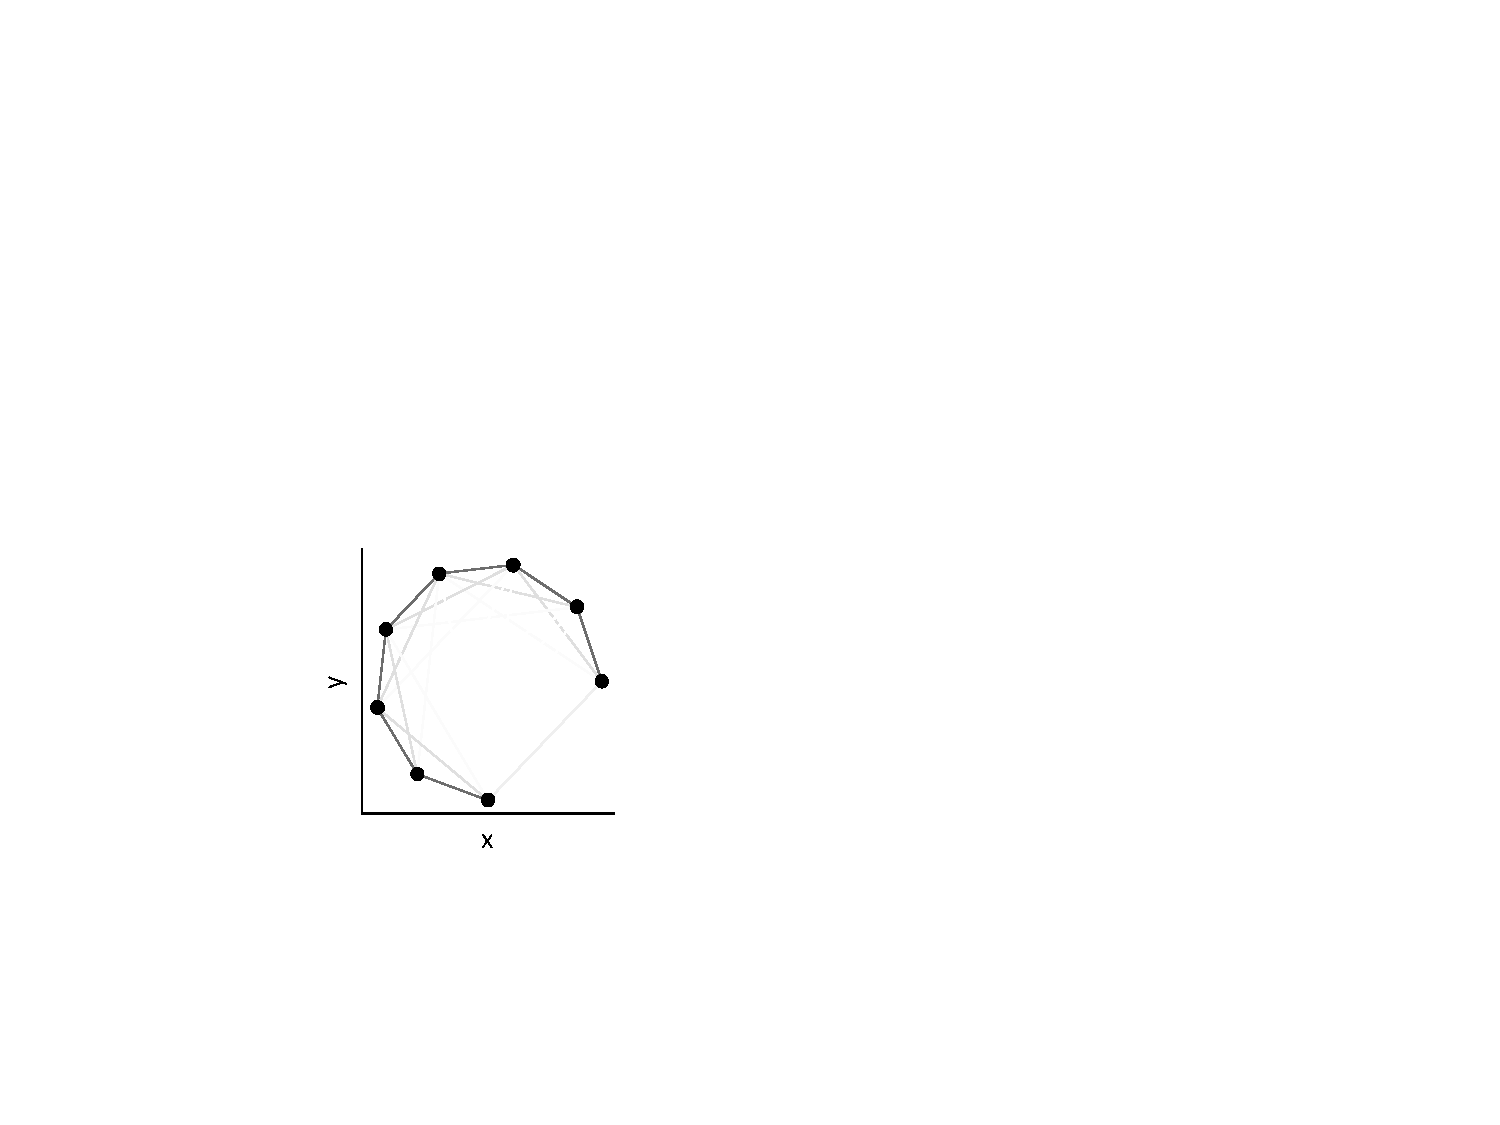
\includegraphics[width=1.5in]{dmaps_edges}};

\node[below=0in of a, align=center, text width=1.5in] (text) {{\scriptsize Illustration of two-dimensional data on a one-dimensional curve. \par}};

\node[right=0.5in of a](b) {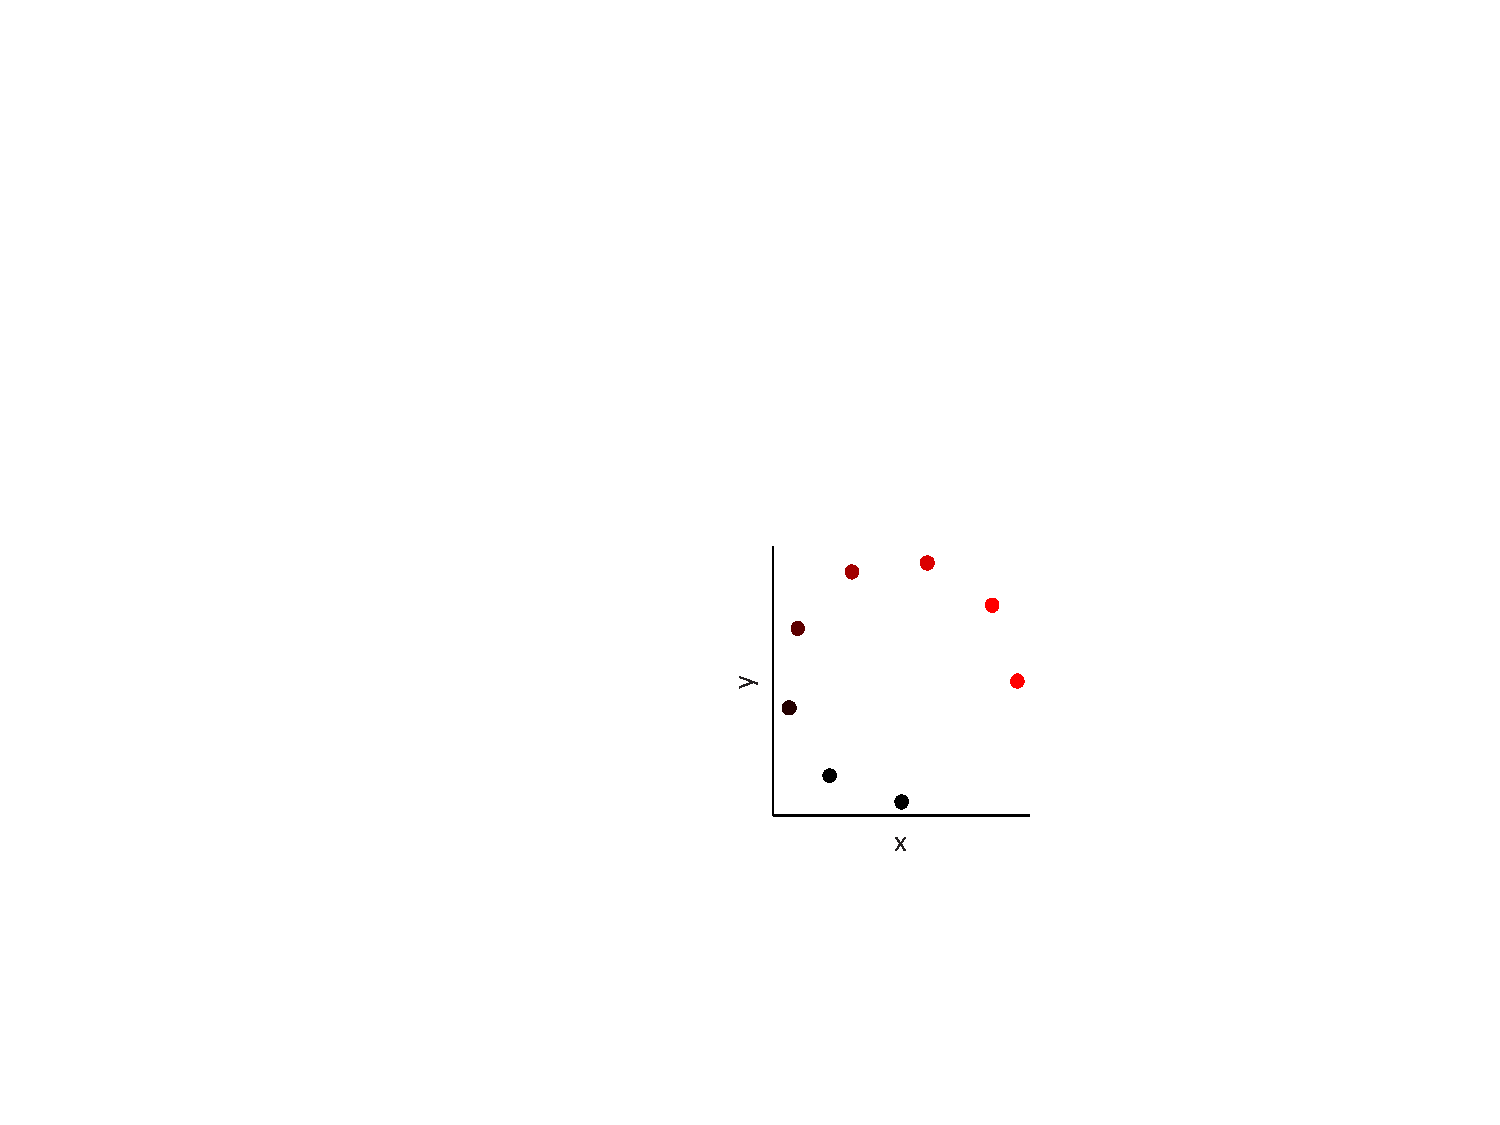
\includegraphics[width=1.5in]{dmaps_color}};

\node[below=0in of b, align=center, text width=1.5in] (text) {{\scriptsize Data, now colored by the one-dimensional parameterization. We assume this parameterization is one-to-one with time. \par}};

\draw[->] (a.east) -- (b.west);
\end{tikzpicture}

\end{center}

\end{frame}

\begin{frame}{Diffusion Maps Algorithm}

\begin{minipage}{0.7\textwidth}

\begin{itemize}

\item Given $m$ data points $x_1, \dots, x_m$, we want to find a coordinate transformation $y(x)$ that preserves local information: points that are close in the original space should also be close in the coordinate $y$.

\item The first step is to construct the matrix $W \in \mathbb{R}^{m \times m}$, where $W_{ij}$ is large if points $x_i$ and $x_j$ are ``close.''
$$W_{ij} = \exp \left( -\frac{d^2(x_i, x_j)}{\epsilon^2} \right)$$
$d(x_i, x_j)$ is the distance between $x_i$ and $x_j$;
$\epsilon$ is a characteristic scale

\end{itemize}
\end{minipage}
\begin{minipage}{0.28\textwidth}
\centering
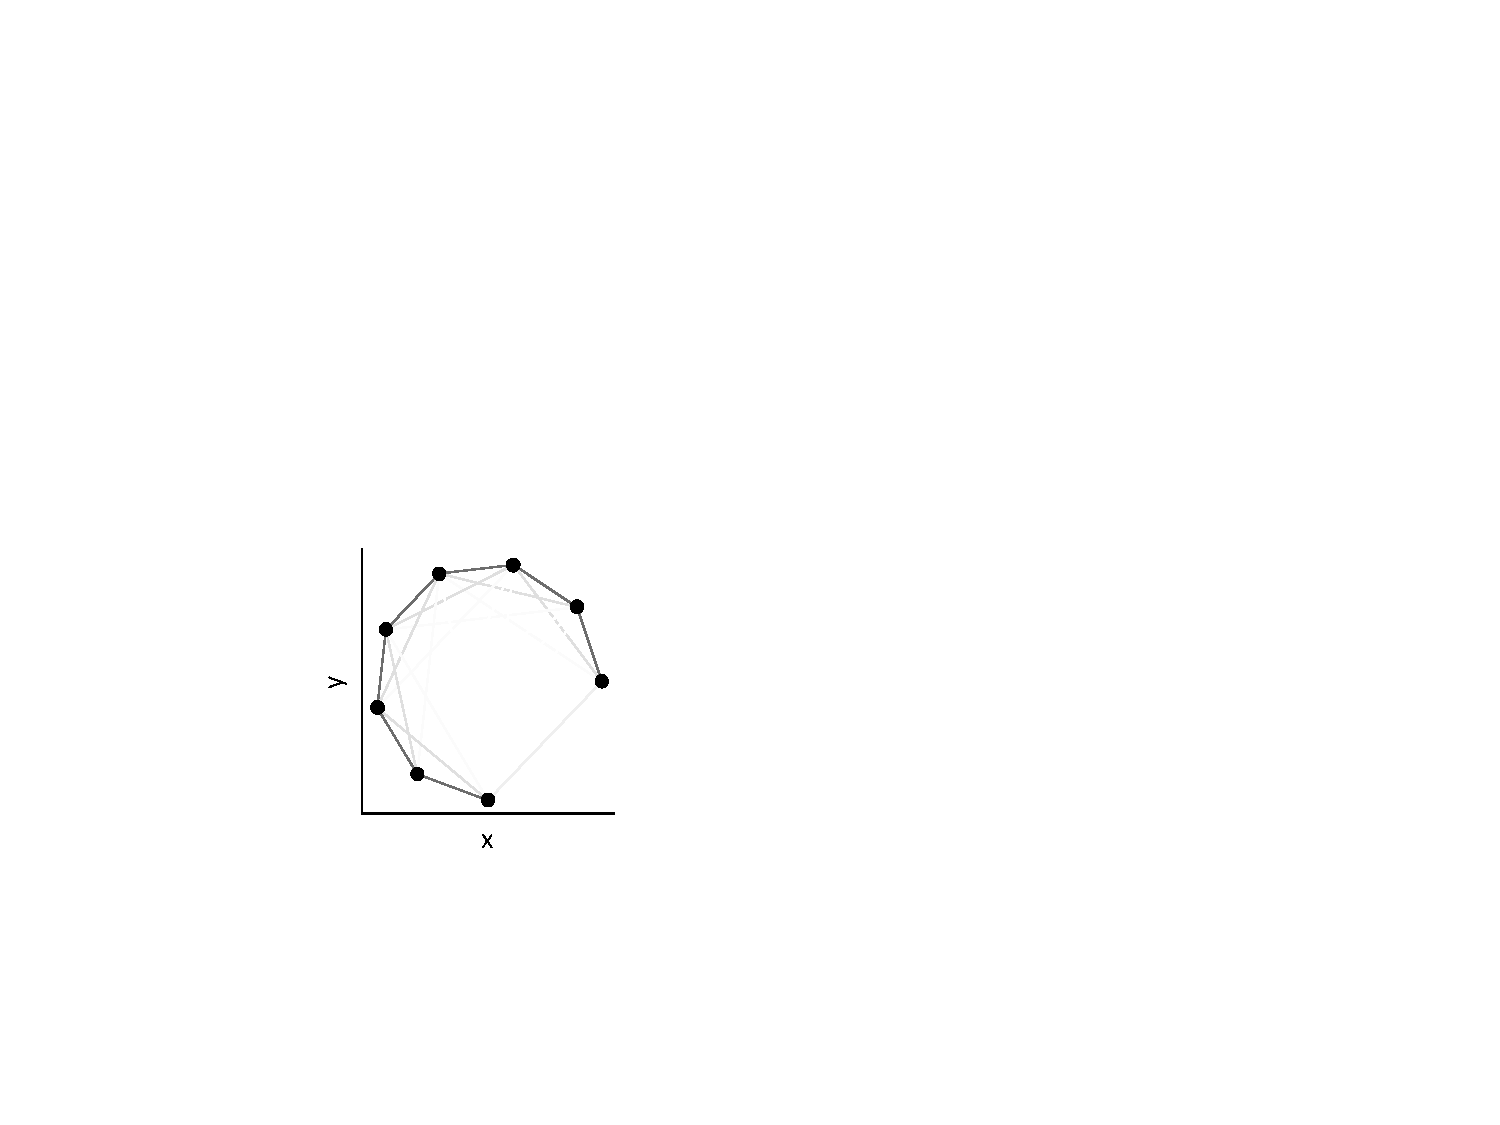
\includegraphics[width=1in]{dmaps_edges}

{\scriptsize Two-dimensional data which lies on a one-dimensional curve. The edge strength is proportional to the kernel $W_{ij}$. \par}
\end{minipage}

\begin{itemize}
\item To find this coordinate $y$, we want solve the following optimization problem \footcite{Belkin2003}
$$\argmin_{y} \sum_{ij} W_{ij} (y(x_i) - y(x_j))^2.$$
%
\item The solution is given by the top (non-trivial) eigenvector of $A$, where $A=D^{-1} W$ and $D$ is a diagonal matrix with $D_{ii} = \sum_{j=1}^{m} W_{ij}$.
%
%\item We have assumed that this single direction of variability is one-to-one with time, and so ordering the data by $y(x_j)$ will then, effectively, order them in time.
%
%\item The procedure generalizes when the data lie on higher-dimensional manifolds (not just curves) in data space.
\end{itemize}

\end{frame}

%\begin{frame}{Temporal Ordering of {\em Drosophila} Images}
%
%
%\begin{center}
%
%\begin{tikzpicture}
%\node(a) {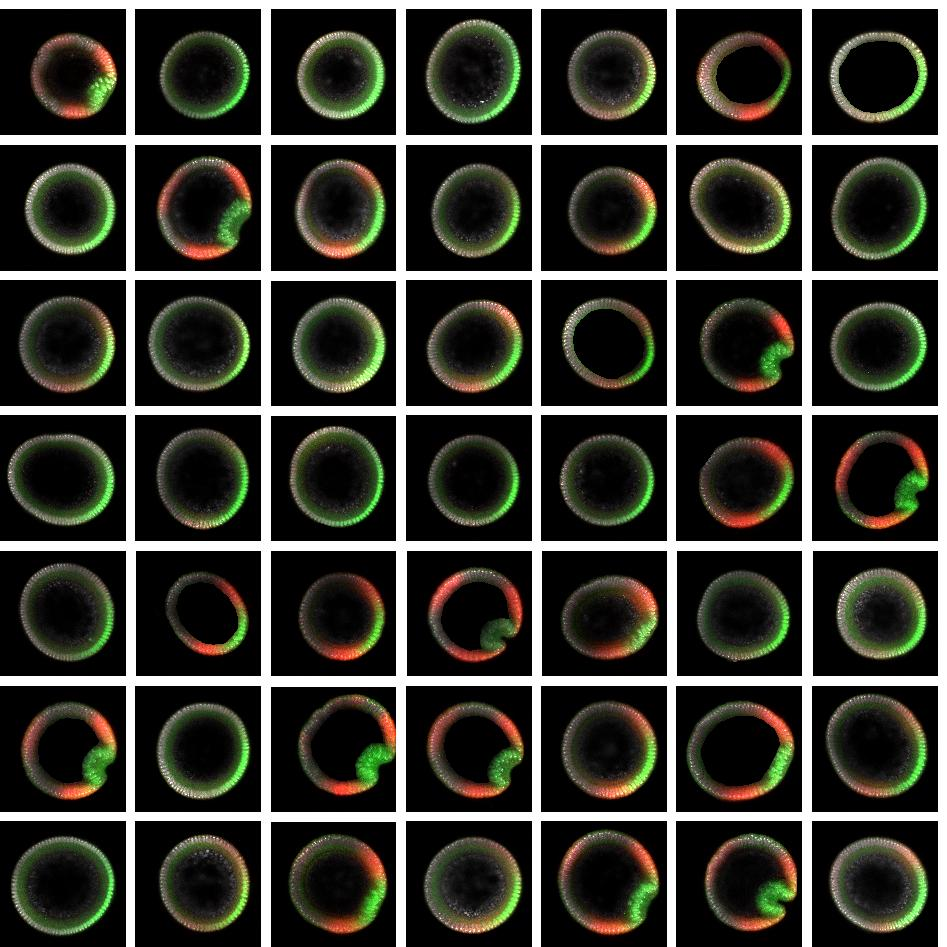
\includegraphics[width=2in]{images_angsynch}};
%
%\node[below=0in of a, align=center, text width=2in](text) {Images, registered using angular synchronization};
%
%\node[right=0.5in of a] (b) {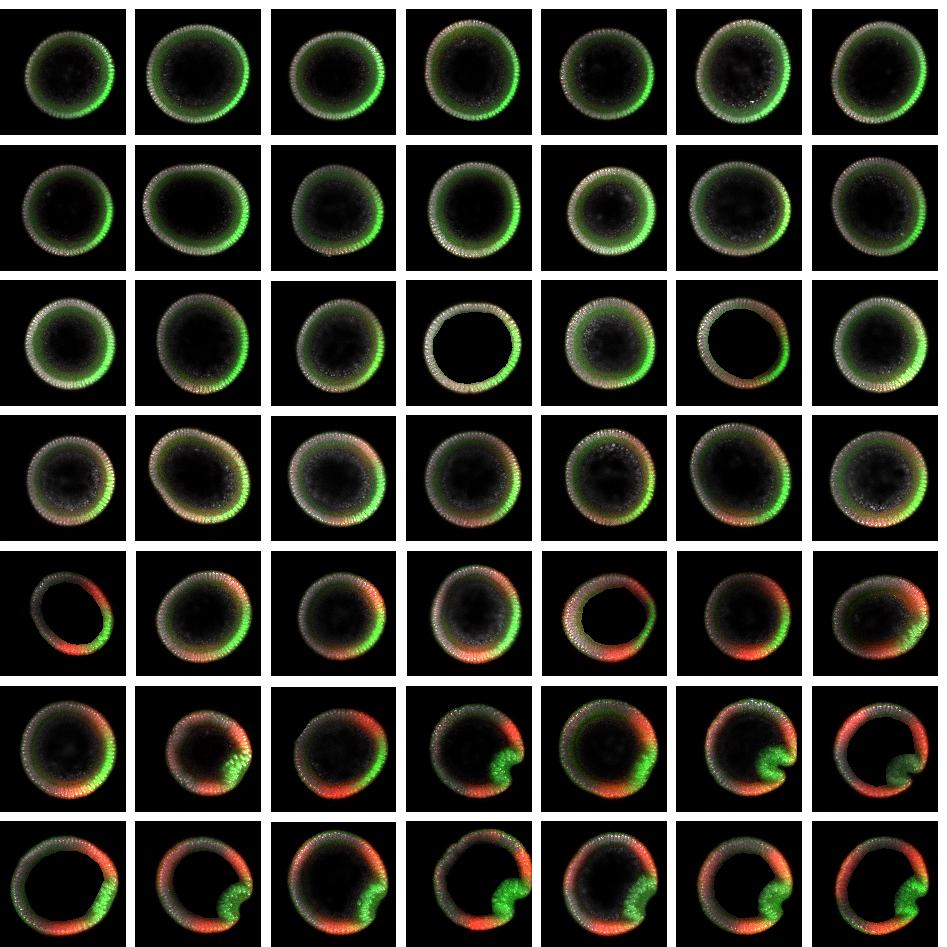
\includegraphics[width=2in]{images_dmaps}};
%
%\node[below=0in of b, align=center, text width=2in](text) {Images, registered using \\angular synchronization and temporally ordered using diffusion maps};
%
%\draw[->] (a.east) -- (b.west);
%
%\end{tikzpicture}
%\end{center}
%
%\end{frame}

\begin{frame}{Combined: Vector Diffusion Maps}



	\begin{minipage}{0.45\textwidth}	
	\begin{block}{Angular Synchronization}
		Calculate top eigenvector of $H$,  
		$$H_{ij} = e^{-i \theta_{ij}}$$
	\end{block}
	\end{minipage}
	\hfill
	\begin{minipage}{0.45\textwidth}
	\begin{block}{Diffusion maps}
		Calculate top eigenvectors of $A$, 
		$$A_{ij} = \frac{\exp \left(-\frac{d^2(x_i, x_j)}{\epsilon^2}\right)}{\sum_j \exp \left(-\frac{d^2(x_i, x_j)}{\epsilon^2}\right)} $$
	\end{block}
	\end{minipage}	
	
	\begin{block}{Vector Diffusion Maps (VDM) \footnotemark} 
		Calculate the top eigenvectors of $S$, where $S_{ij} = A_{ij}H_{ij}$
		
	\end{block}
	\footcitetext{singer2012vector}

\begin{itemize}
\item The top eigenvector(s) of $S$ give us the optimal alignments/rotations for our images
\item Successive eigenvectors give us the embedding coordinates/temporal ordering for our images
\end{itemize}

\end{frame}

\begin{frame}{Registration and Ordering of Images Using Vector Diffusion Maps}

\begin{center}

\begin{tikzpicture}
\node(a) {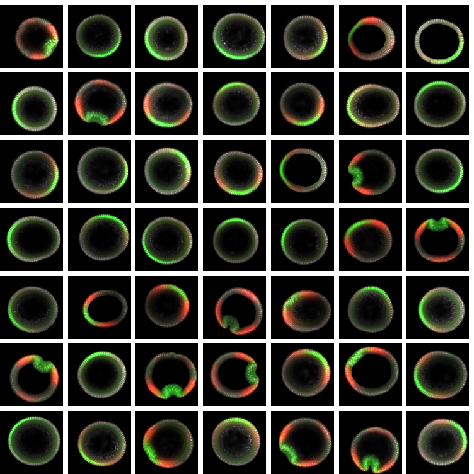
\includegraphics[width=2in]{fig2a}};

\node[below=0in of a, align=center, text width=2in](text) {Images, unregistered and unordered};

\node[right=0.5in of a] (b) {\includegraphics[width=2in]{VDM_data1_ordered}};

\node[below=0in of b, align=center, text width=2in](text) {Images, registered and ordered using vector diffusion maps};

\draw[->] (a.east) -- (b.west);

\end{tikzpicture}
\end{center}

\end{frame}

\begin{frame}{Validating Registration and Temporal Ordering}

\centering

For this particular system, both registration and temporal ordering can be done using prior  knowledge 

\vspace{0.1in}

\begin{minipage}{0.35\textwidth}
\begin{center}
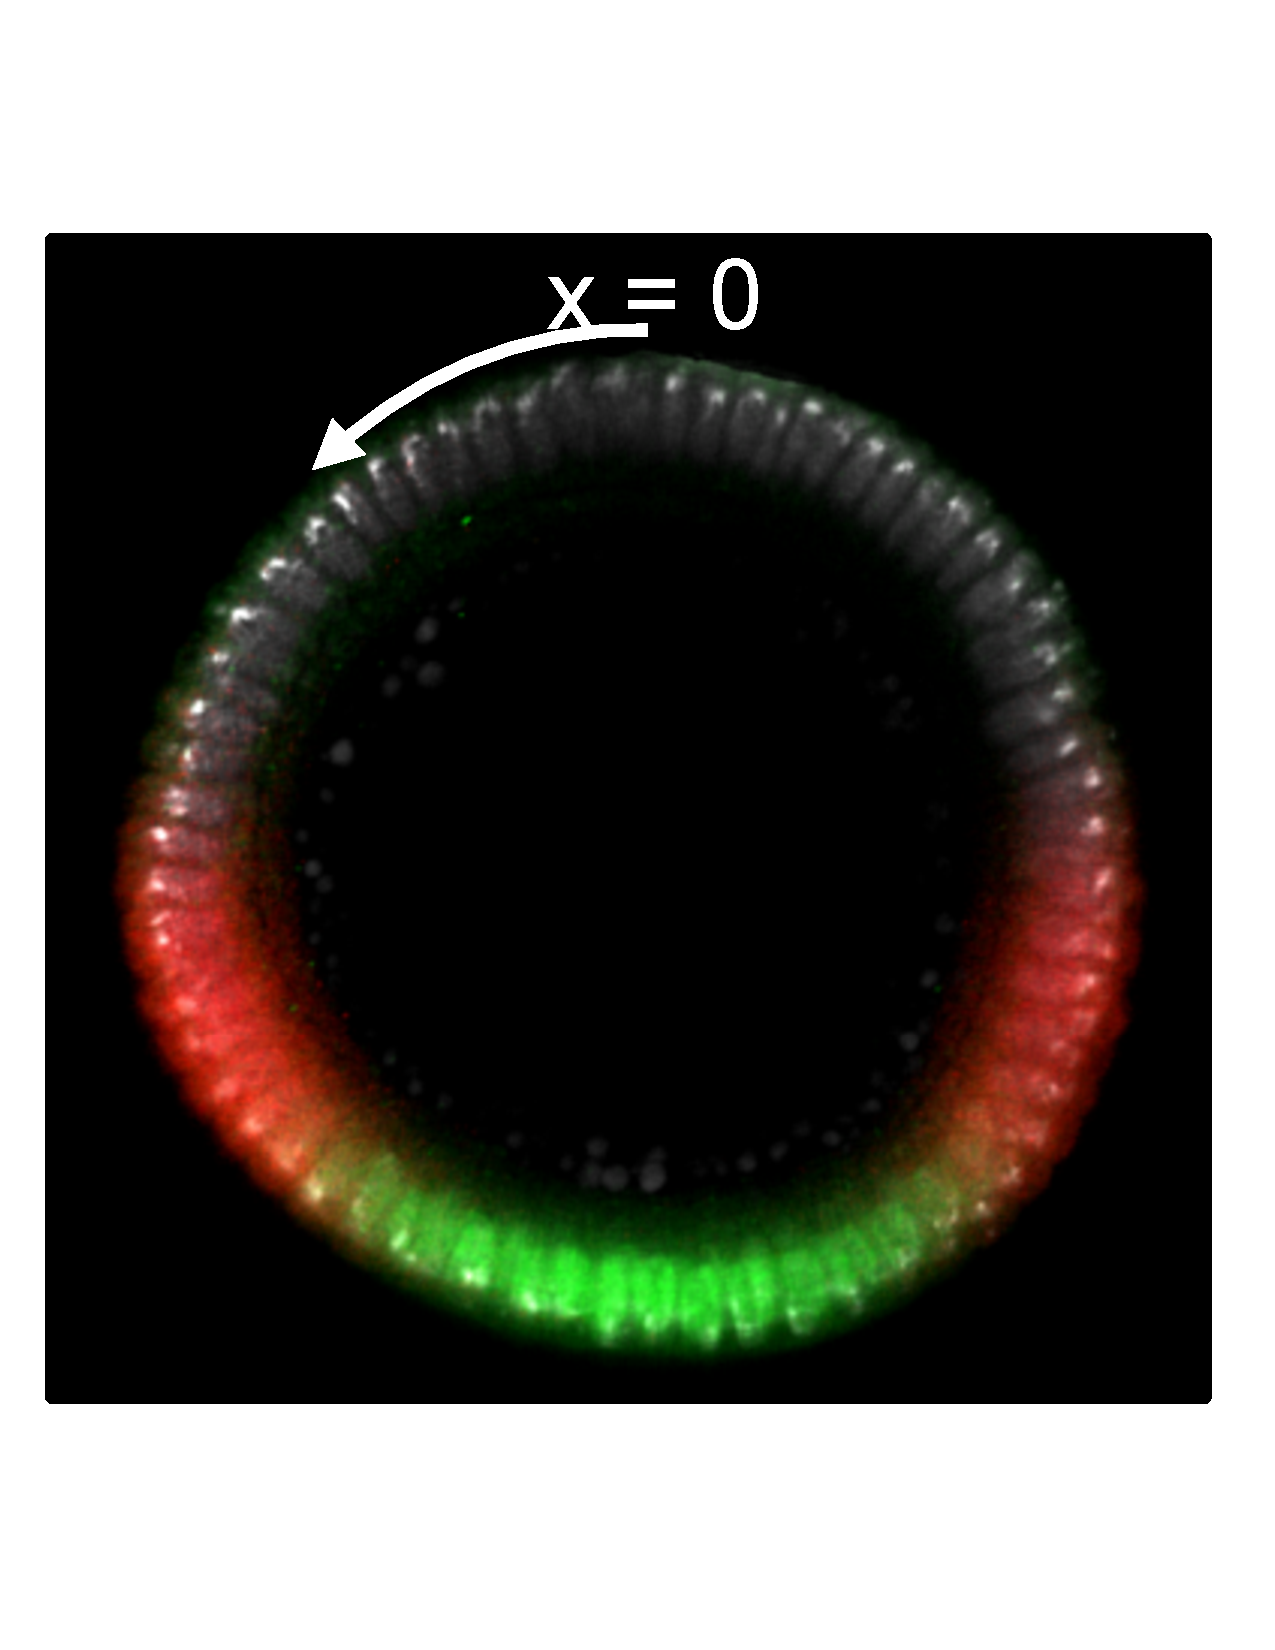
\includegraphics[width=1in]{one_embryo}

{\small 
\textcolor{bold}{Registration:} The green peak specifies the ventralmost point of the embryo

\par}

\end{center}
\end{minipage}
\hfill
\begin{minipage}{0.6\textwidth}

\begin{center}
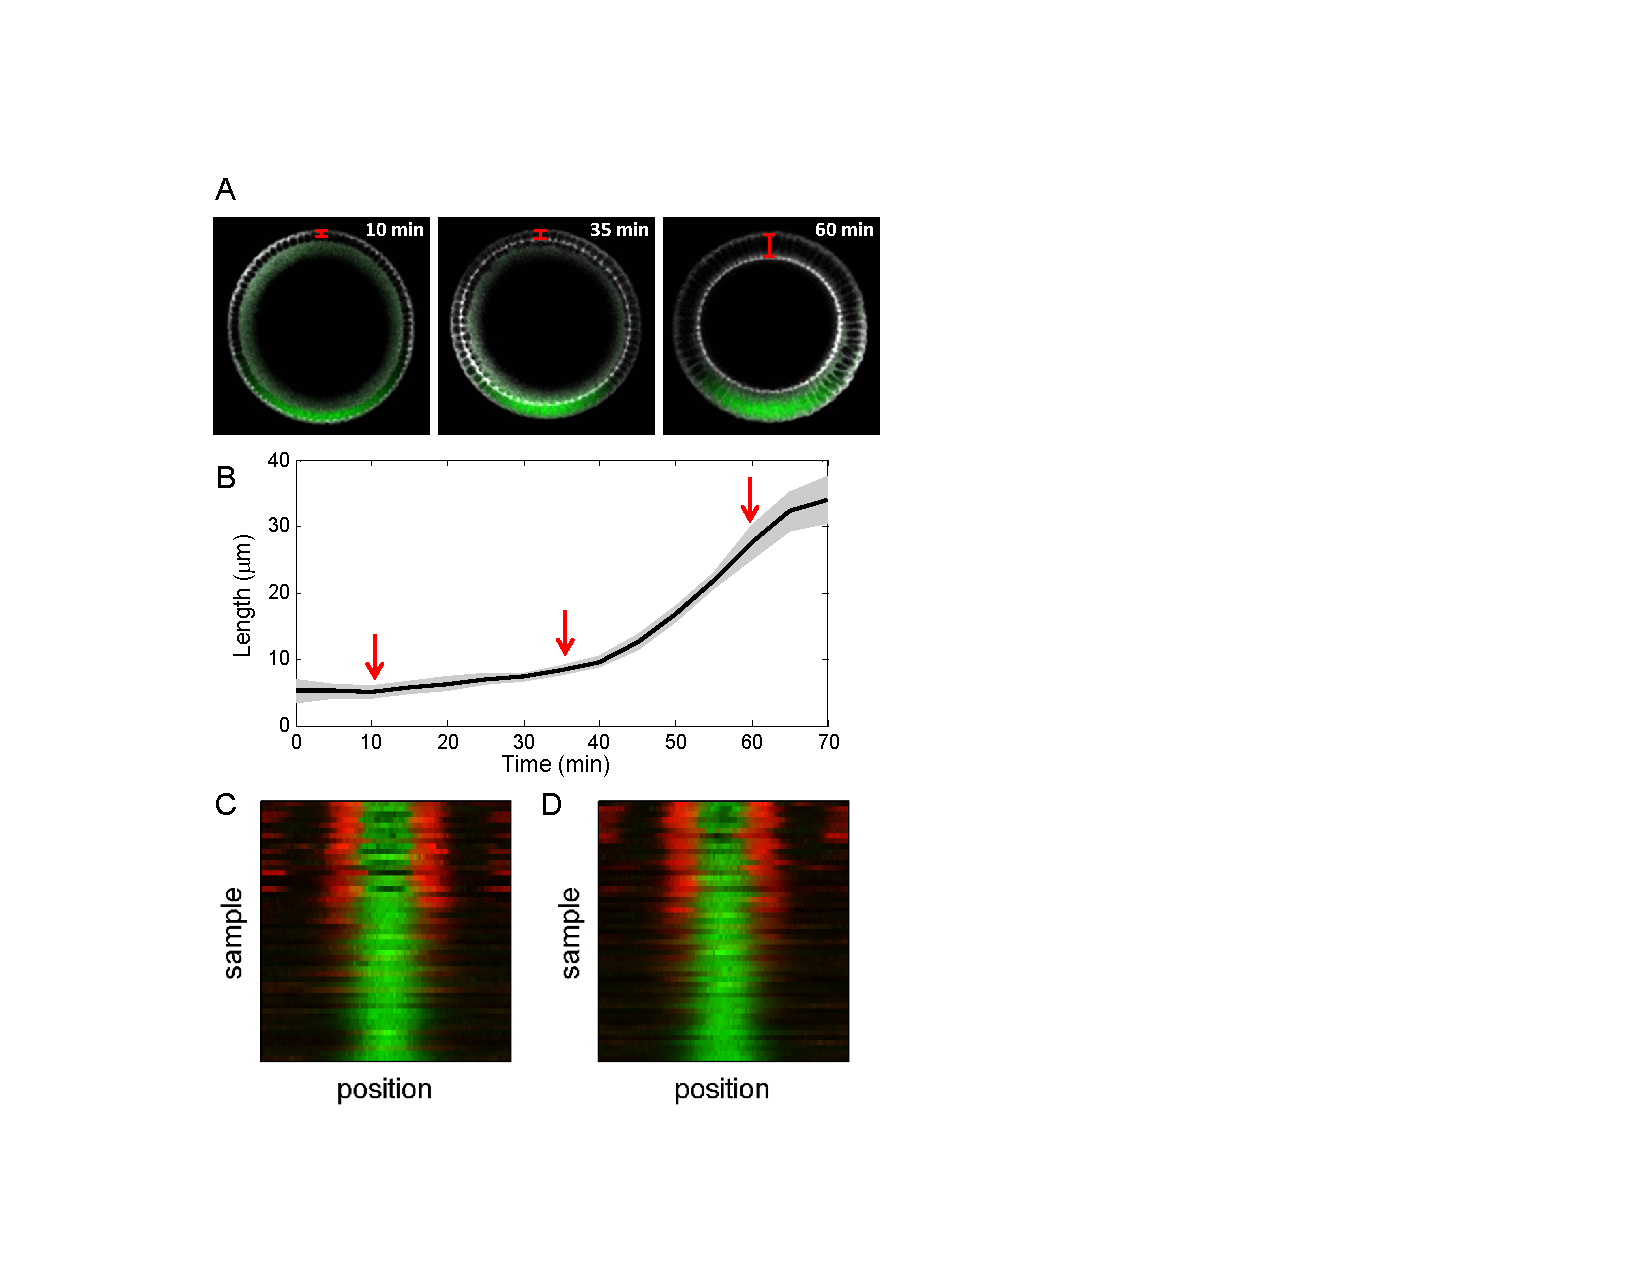
\includegraphics[width=2in, trim=0in 2.2in 0in 0in, clip]{fig6}

{\small 
\textcolor{bold}{Ordering:} 
Membranes grow in thickness \\as a function of time \footnotemark \par}

{\em \scriptsize Note that the curve becomes flatter and noisier \\at the end of the developmental time window \par}

\end{center}
\end{minipage}

\footcitetext{figard2013plasma}

\end{frame}


\begin{frame}{Validation of Automatic Registration and Ordering}


\begin{center}

We compare concentration profiles around the circumference of the embryo

\begin{tikzpicture}

\node(a){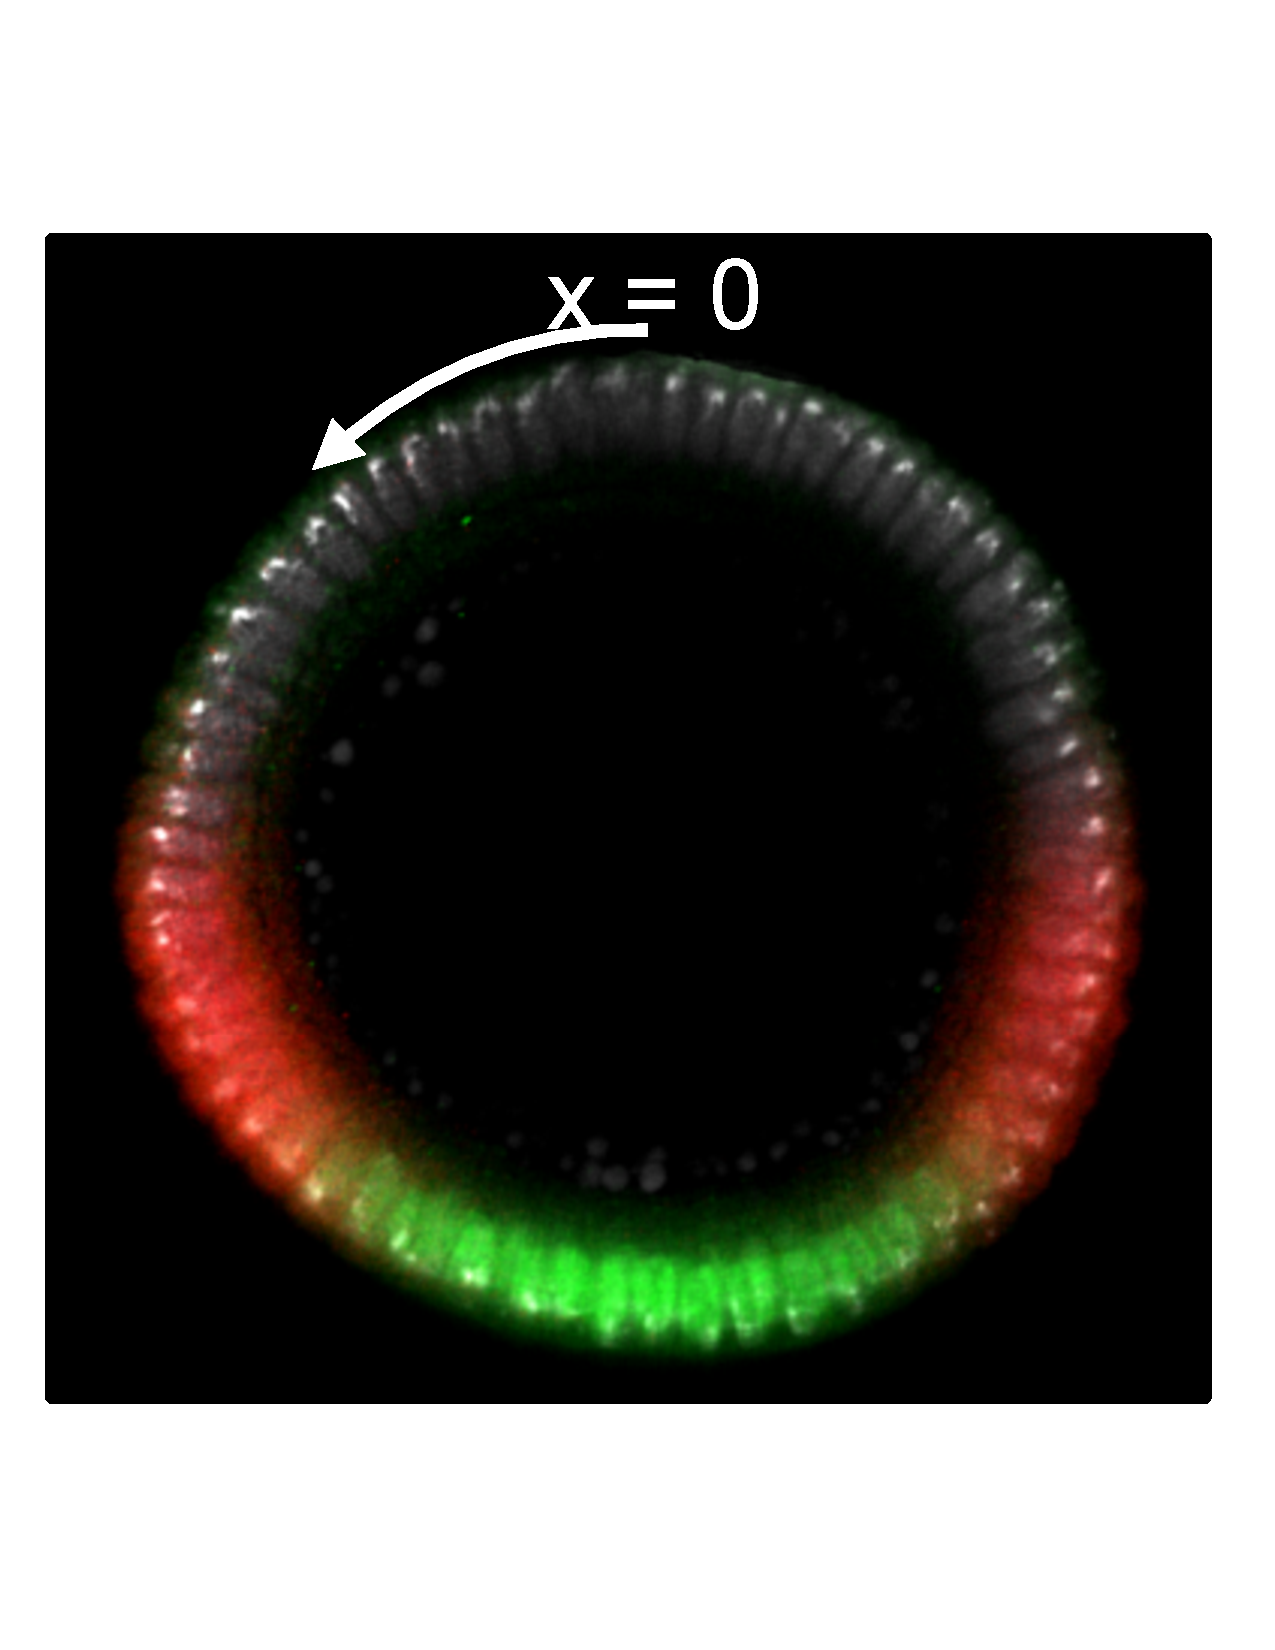
\includegraphics[width=0.8in]{one_embryo}};
\node[right=0.5in of a](b) {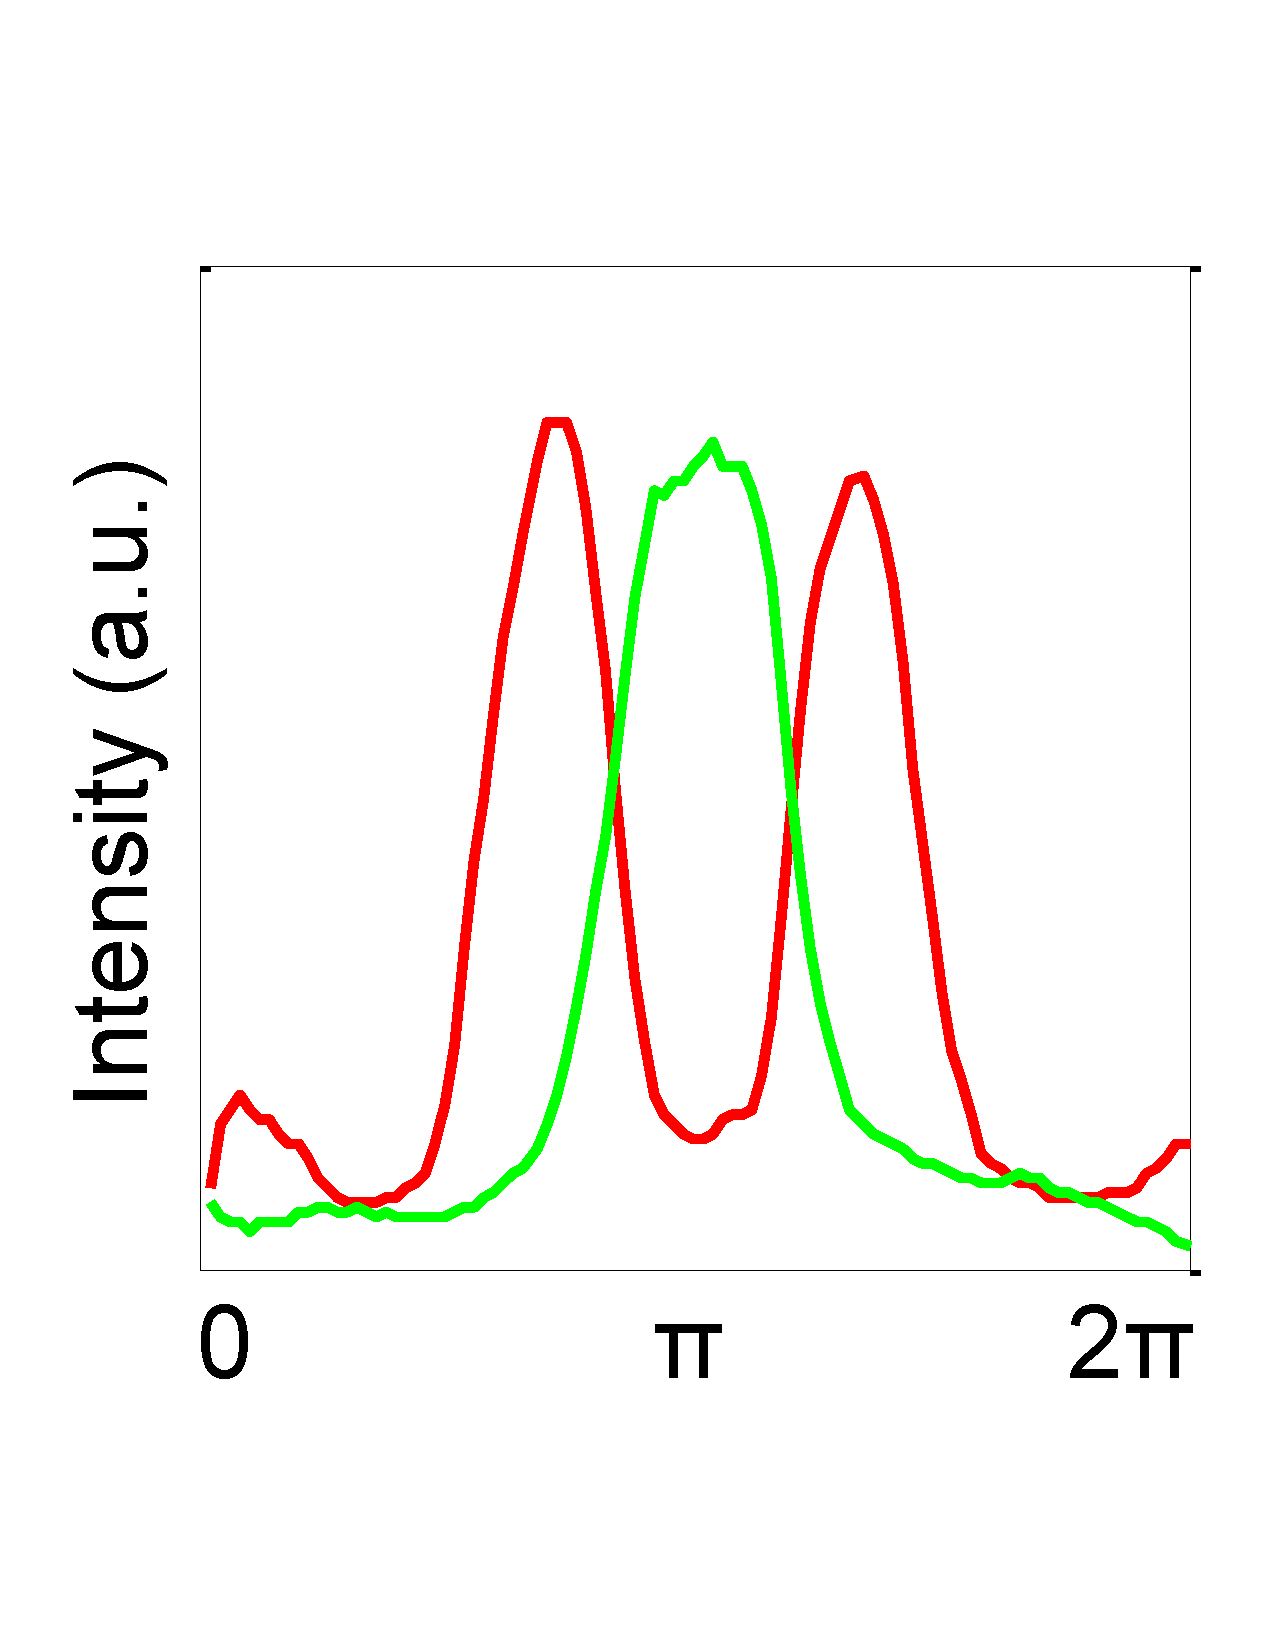
\includegraphics[width=0.8in, trim=0in 0.1in 0in 0in, clip]{fig2c}};

\draw[->](a.east) -- (b.west);
\end{tikzpicture}

\end{center}

\centering
\begin{minipage}{3.1in}
\centering
The results appear consistent 

\begin{minipage}{1.3in}
\centering
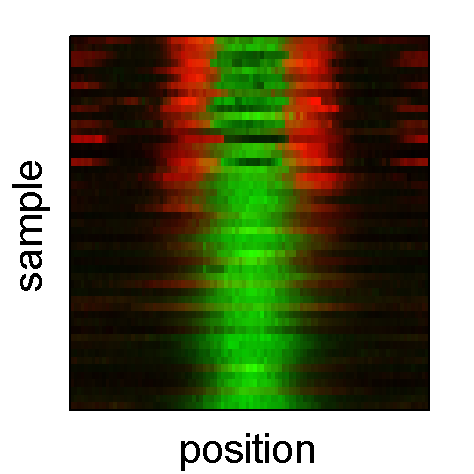
\includegraphics[width=1in]{fig6b}\\
{\scriptsize Registered using green peaks \\
Ordered using membranes \par}
\end{minipage}
%
\begin{minipage}{1.3in}
\centering
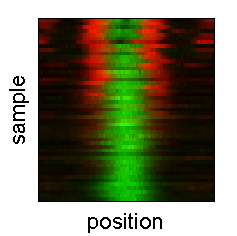
\includegraphics[width=1in]{fig6c}\\
{\scriptsize Registered and ordered using vector diffusion maps \par}
\end{minipage}
\end{minipage}
\hspace{0.5in}
\begin{minipage}{1.5in}
\centering
Rank correlation
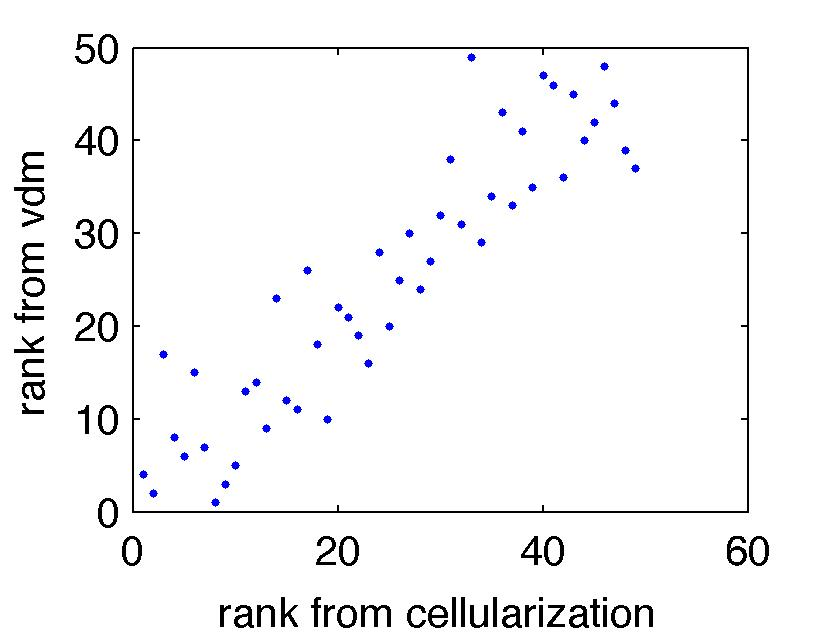
\includegraphics[width=1.4in]{rank_corr_vdm}\\
$\rho=0.9158$
\end{minipage}

\end{frame}

\section{Ordering Images From Gastrulation}

\begin{frame}{Registering and Ordering a More Complex Data Set}

\centering

Following cellularization, there is gastrulation, when the embryos begin to morph and deform. 

\begin{tikzpicture}

\node (a) {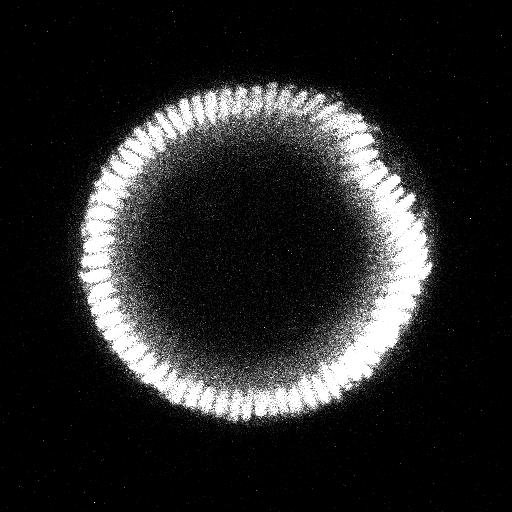
\includegraphics[width=0.5in]{emb02_hisRFP_gastrulation10}};
\node[below=0in of a] (text) {{\scriptsize 0~min}};

\node[right=0in of a] (a) {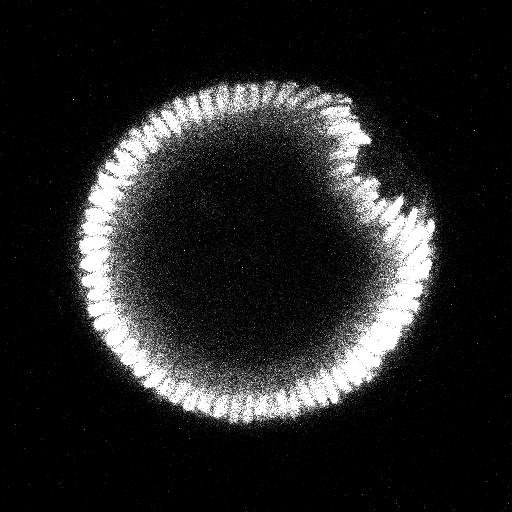
\includegraphics[width=0.5in]{emb02_hisRFP_gastrulation15}};
\node[below=0in of a] (text) {{\scriptsize 2.5~min}};

\node[right=0in of a] (a) {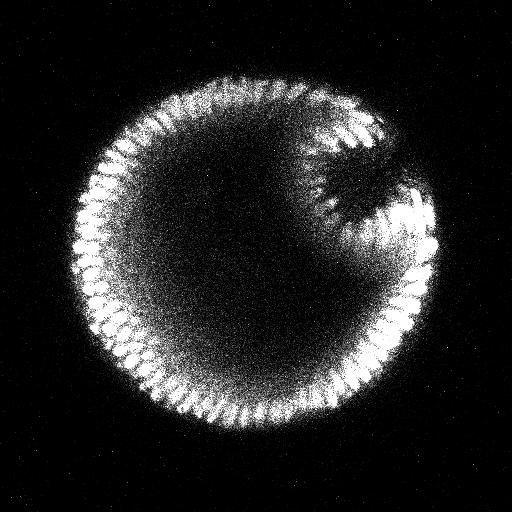
\includegraphics[width=0.5in]{emb02_hisRFP_gastrulation20}};
\node[below=0in of a] (text) {{\scriptsize 5~min}};

\node[right=0in of a] (a) {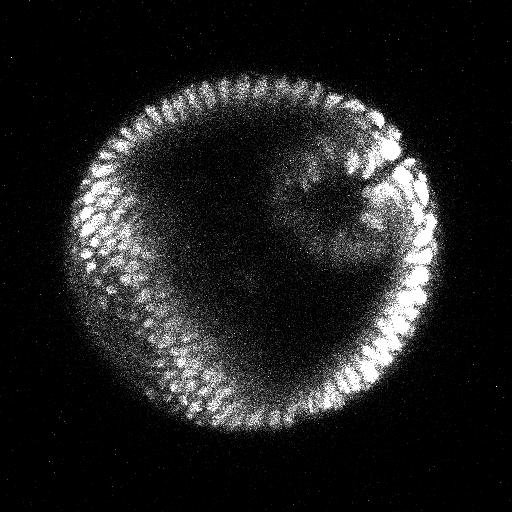
\includegraphics[width=0.5in]{emb02_hisRFP_gastrulation25}};
\node[below=0in of a] (text) {{\scriptsize 7.5~min}};

\node[right=0in of a] (a) {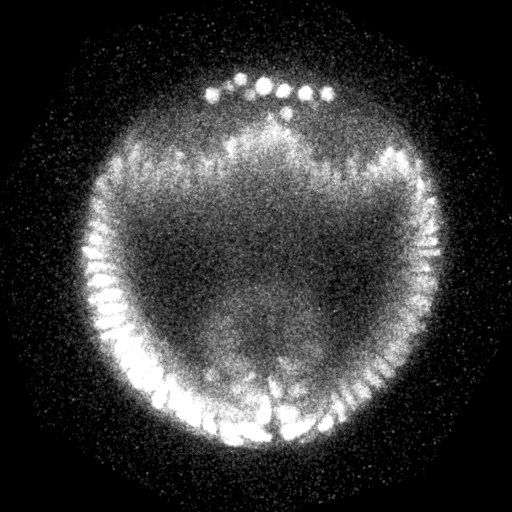
\includegraphics[width=0.5in]{emb02_hisRFP_gastrulation30}};
\node[below=0in of a] (text) {{\scriptsize 10~min}};

\node[right=0in of a] (a) {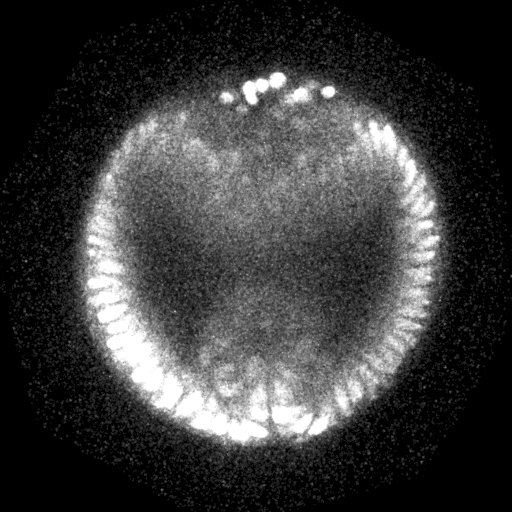
\includegraphics[width=0.5in]{emb02_hisRFP_gastrulation35}};
\node[below=0in of a] (text) {{\scriptsize 12.5~min}};

\node[right=0in of a] (a) {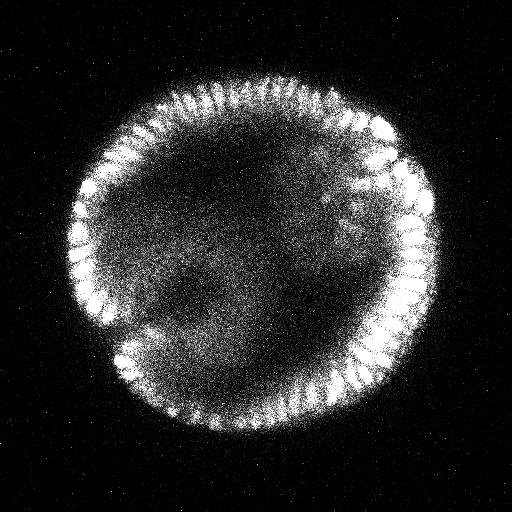
\includegraphics[width=0.5in]{emb02_hisRFP_gastrulation40}};
\node[below=0in of a] (text) {{\scriptsize 15~min}};

\node[right=0in of a] (a) {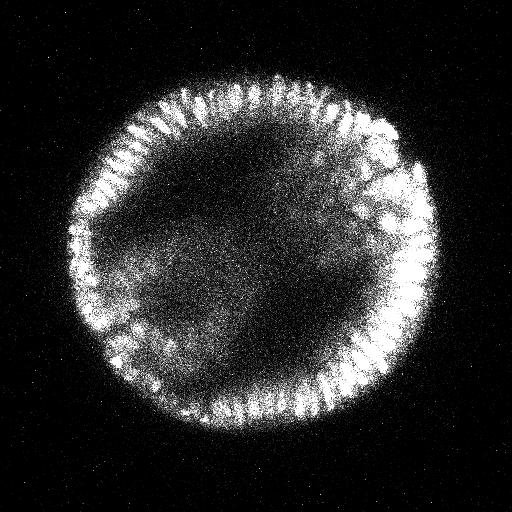
\includegraphics[width=0.5in]{emb02_hisRFP_gastrulation45}};
\node[below=0in of a] (text) {{\scriptsize 17.5~min}};

%\node[right=0in of a] (a) {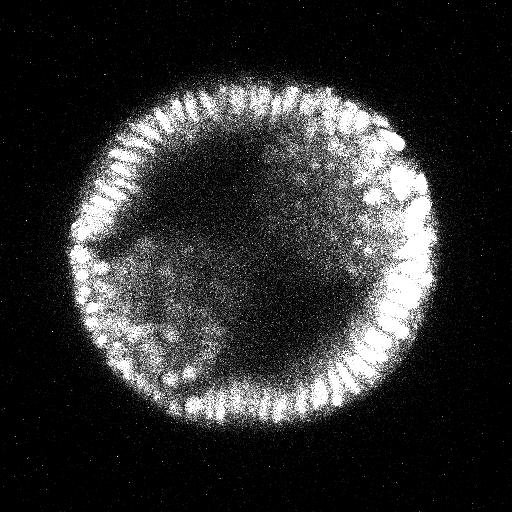
\includegraphics[width=0.5in]{emb02_hisRFP_gastrulation49}};
%\node[below=0in of a] (text) {{\scriptsize 20~min}};

\end{tikzpicture}

During this time period, we have no good way to accurately measure the time of fixed images.

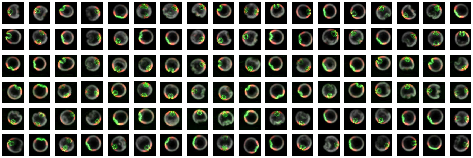
\includegraphics[width=0.7\textwidth]{raw_data2}

We want to register and temporally order this data.

\end{frame}

\begin{frame}{Registered and Ordered using VDM}

\centering

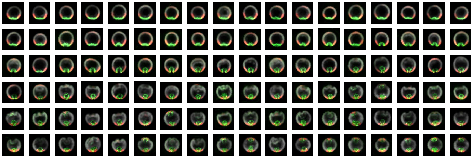
\includegraphics[width=0.8\textwidth]{VDM_ordered}

The data has now been registered and ordered using VDM

\vspace{0.1in}

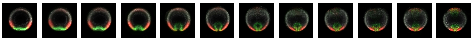
\includegraphics[width=\textwidth]{average_trajectory}

We can compute an {\em average} developmental trajectory.
\end{frame}

\section{Conclusions}

\begin{frame}{Conclusions}

\begin{itemize}
\item In many experiments, we are presented with cross-sectional imaging data that must be registered and temporally ordered
\item Both of these tasks can be automated, using angular synchronization (for registration), diffusion maps (for temporal ordering), and vector diffusion maps (for simultaneous registration + ordering)
\item In the first example, we have independent time and space markers, and we can validate our automatic methods
\item We are now interested in matching fixed images with {\em live movies} that contain only one signal (e.g., nuclei) so that we can determine the rates of relevant developmental processes
\end{itemize}

\vspace{0.5in}
\begin{center}
{\Large Thank you to CSGF and Krell!}


\includegraphics[width=2in]{CSGF_horiz_1200x360}
\end{center}


\end{frame}

\end{document}
